\subsection{Lidar Mount}
% Design reqs: needed to rigidly attach to Nao for data transformation purposes, needed to see forward,
% lightweight, Nao needed to be able to move his head while wearing it,
% needed to be able to use the sonars (just in case).
In order to attach the URG Lidar to the Nao a custom Lidar mount was built.
The mount needed to hold the Lidar such that obstacles in front of the robot
could be sensed. It had to be lightweight, rigidly attached, and allow
the robot to move its head to track the red cube. Finally, it should not inhibit
the use of the sonars, in the event that the sonars are used in the future.

% Mounting it to the head seemed like it was going to be tough, so a vest was designed.
% Straps and foam seemed like they'd hold well enough. In fact they hold so well I can lift Nao up by the mount.
% The mount was made from PLA, 3D printer, foam, velcro straps.
The Lidar mount was designed as a tray positioned at waist-height, 
in the front of the robot.
As the Nao is not equipped with any mounting points, it was attached
using straps. The rigid parts were manufactured out of PLA plastic using a 3D
printer. The printed parts that would contact the robot were padded with foam to
create a surface that would conform to the Nao's body and hold securely.
Figure~\ref{fig:nao_lidar_mount_nao_dimetric1} shows a CAD model of the finished
assembly.

\begin{figure}
\centering
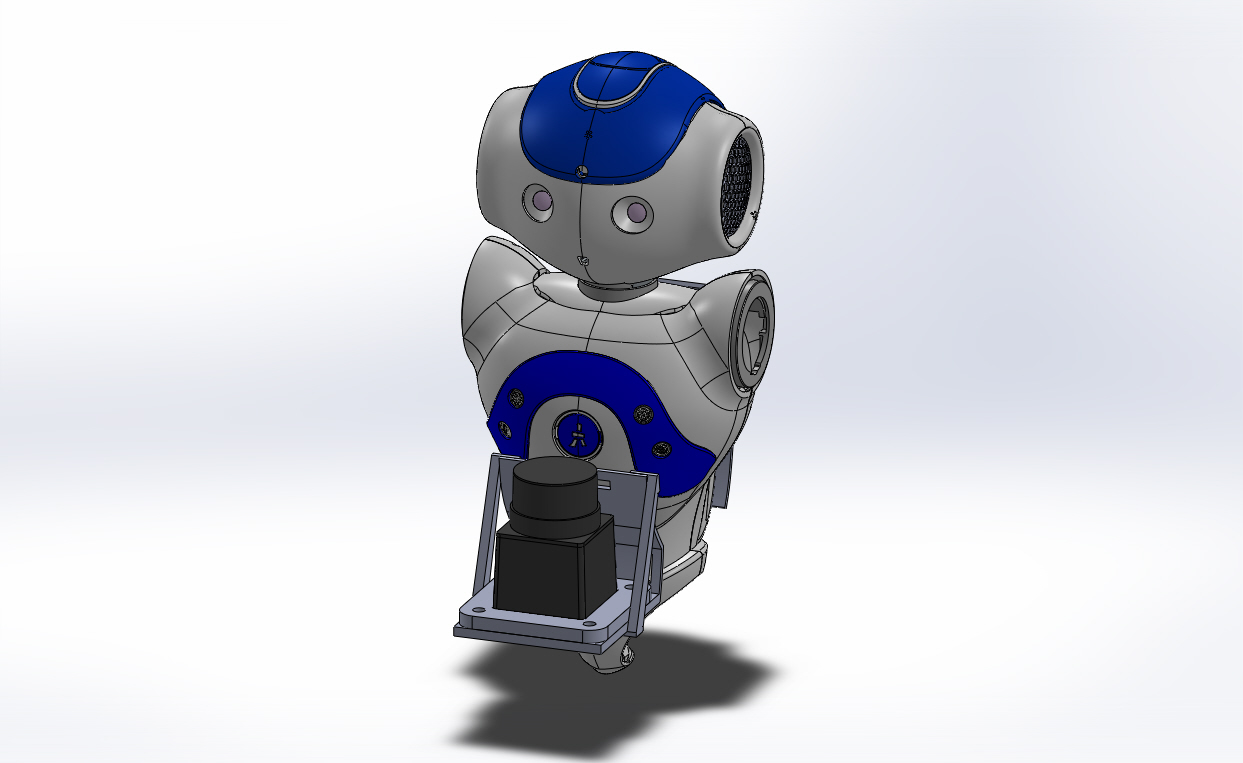
\includegraphics[height=0.3\textheight]{backpack/Assem_Nao_Dimetric1.jpg}
\caption{CAD model of Nao with Hokuyo URG-04LX-UG01 mounted
         to the waist of the robot using a custom mount.}
\label{fig:nao_lidar_mount_nao_dimetric1}
\end{figure}

The mount consisted of two major parts, the front subassembly and the back plate.
The front subassembly held the Lidar to the Nao at waist height, and the back plate
provided a place to anchor the straps from the front. Both pieces sandwiched the
chest of the Nao to create a tight jacket that the robot would carry.
A picture of the assembly mounted to the robot can be seen in
Figure~\ref{fig:nao_lidar_mount_picture1} which shows the straps over the
shoulder of the robot and around the waist.

\begin{figure}
\centering
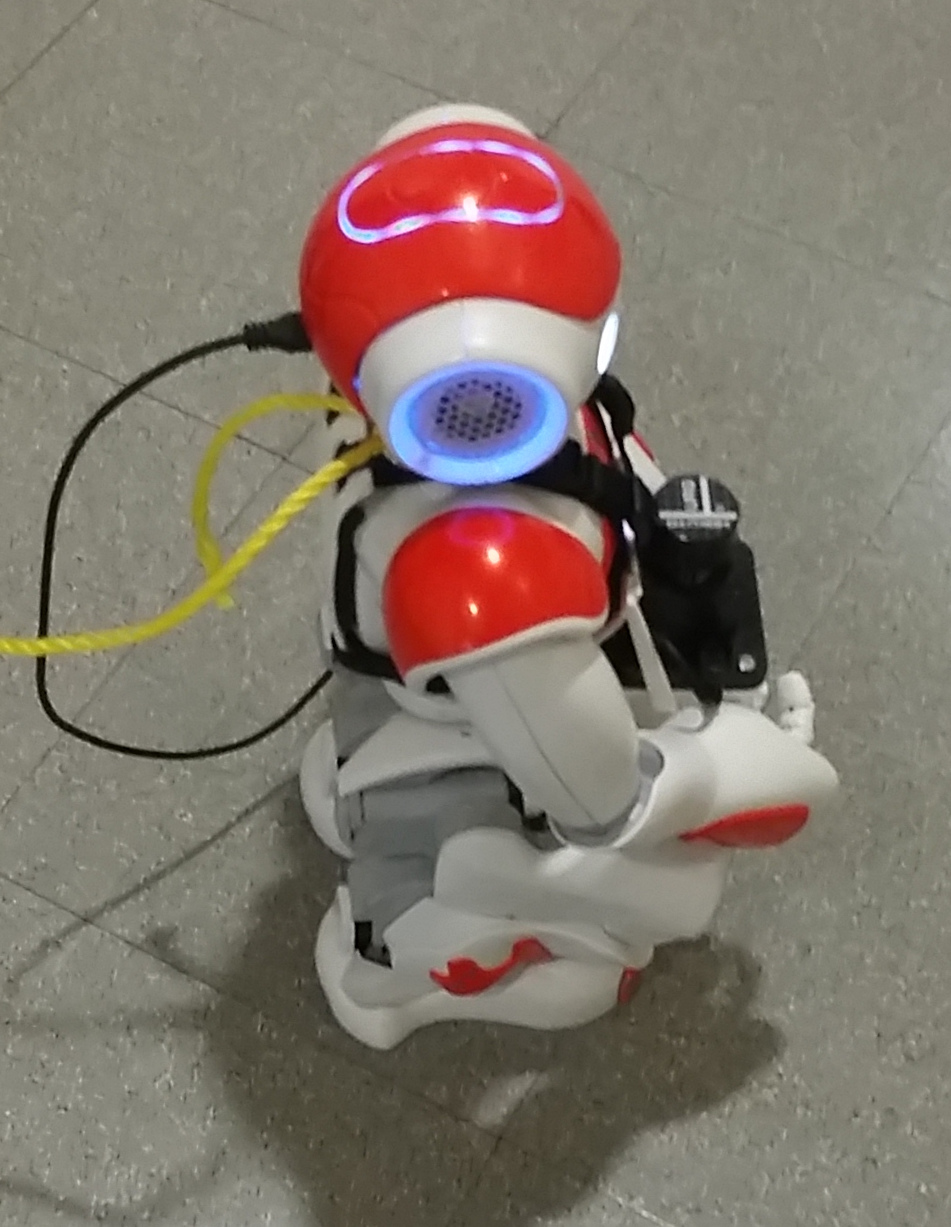
\includegraphics[height=0.3\textheight]{backpack/nao_with_mount2.jpg}
\caption{Photograph of the URG mounted to the Nao using the
         custom Lidar mount.}
\label{fig:nao_lidar_mount_picture1}
\end{figure}

Figure~\ref{fig:nao_lidar_mount_nao_three_view1} shows the back, front, and
side view of the CAD model of the Lidar mount with the URG, torso, and head of the
Nao. The back view shows the back plate which is an anchor for the straps.
The front view shows the front subassembly holding the URG\@. The side view
shows how these pieces conform to the shape of the robot. One set of straps
go from the front of the front subassembly to the back plate, while the second set
go around the waist. When installed, they form a tight sandwich that can support
the weight of the robot.

\begin{figure}
\centering
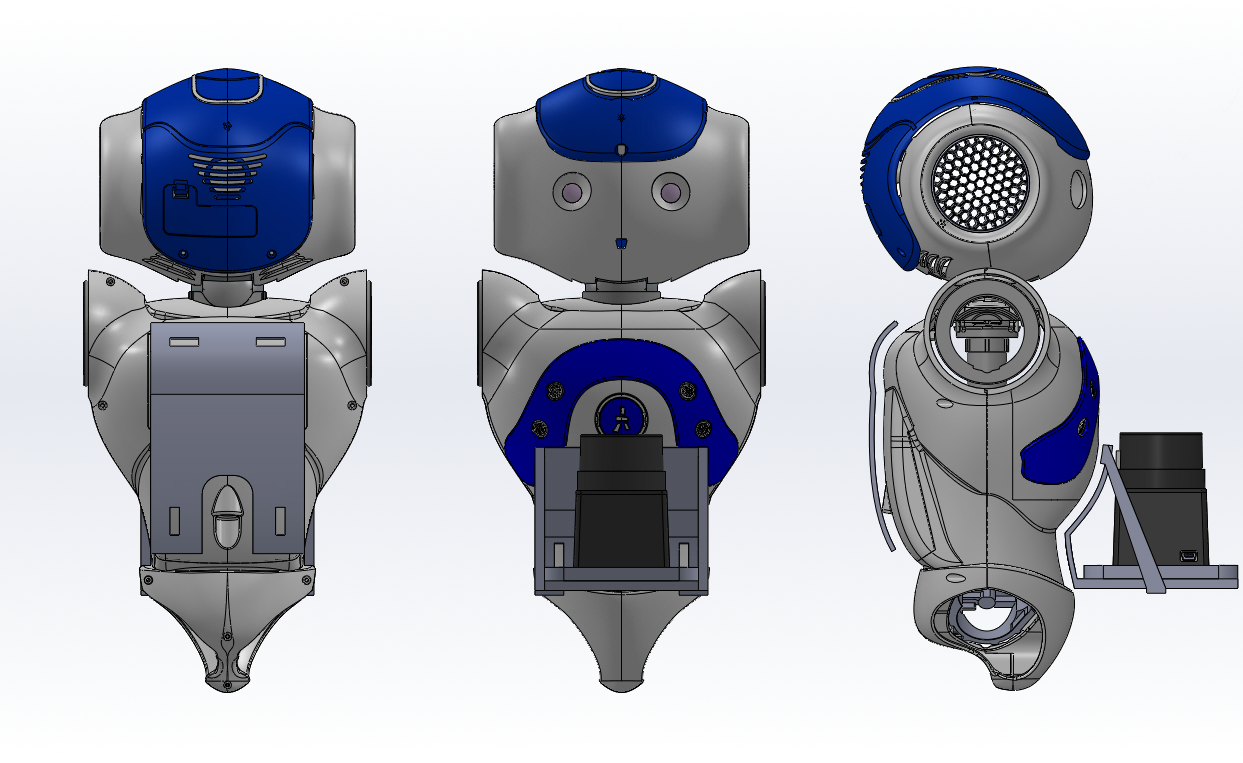
\includegraphics[height=0.3\textheight]{backpack/Assem_Nao_Three_View1.png}
\caption{Back, front, and side views of the URG CAD model 
         mounted to the Nao using the custom mount.}
\label{fig:nao_lidar_mount_nao_three_view1}
\end{figure}

\FloatBarrier

\subsubsection{Front Subassembly}
The front subassembly of the Lidar mount consists of three parts: a front plate,
a base plate, and side supports. Figure~\ref{fig:nao_lidar_mount_dimetric1}
shows a CAD model of the assembled front subassembly with the URG installed.

\begin{figure}[H]
\centering
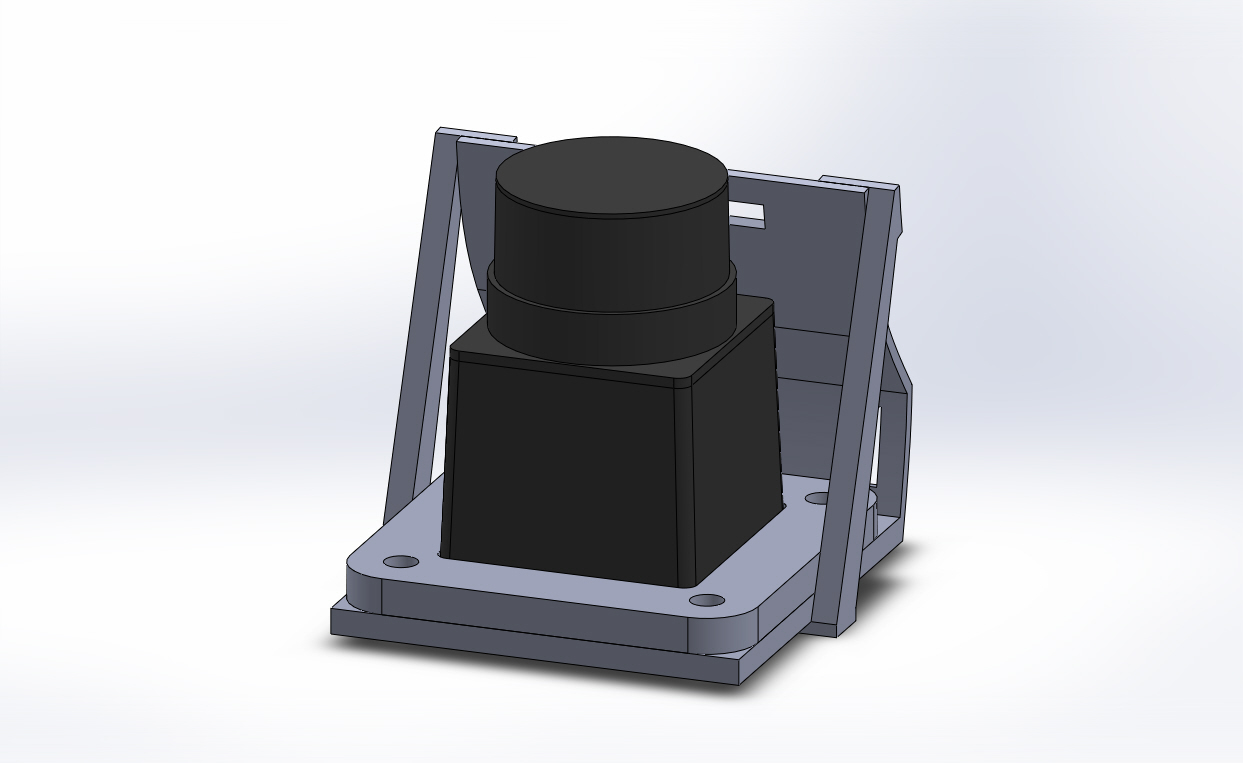
\includegraphics[height=0.25\textheight]{backpack/Assem_FrontOnly_Dimetric1.jpg}
\caption{CAD model of the URG attached to the front subassembly
         of the custom Lidar mount.}
\label{fig:nao_lidar_mount_dimetric1}
\end{figure}

The front plate interfaces with the surface of the robot and provides the
holes for the straps. It also has a flat platform that acts like a tray which protrudes from the
waist of the robot to carry the base plate. The base plate holds the URG
and attaches to the front plate platform. Two side supports act as gussets
to reinforce the tray and to discourage bending.
Figure~\ref{fig:nao_lidar_mount_three_view1} shows the back, front, and side
views of the assembly. The back view shows the holes for the straps, 
while the side view shows the front plate curvature that conforms
to the shape of the robot. The side supports can also be seen in the side view.

\begin{figure}[H]
\centering
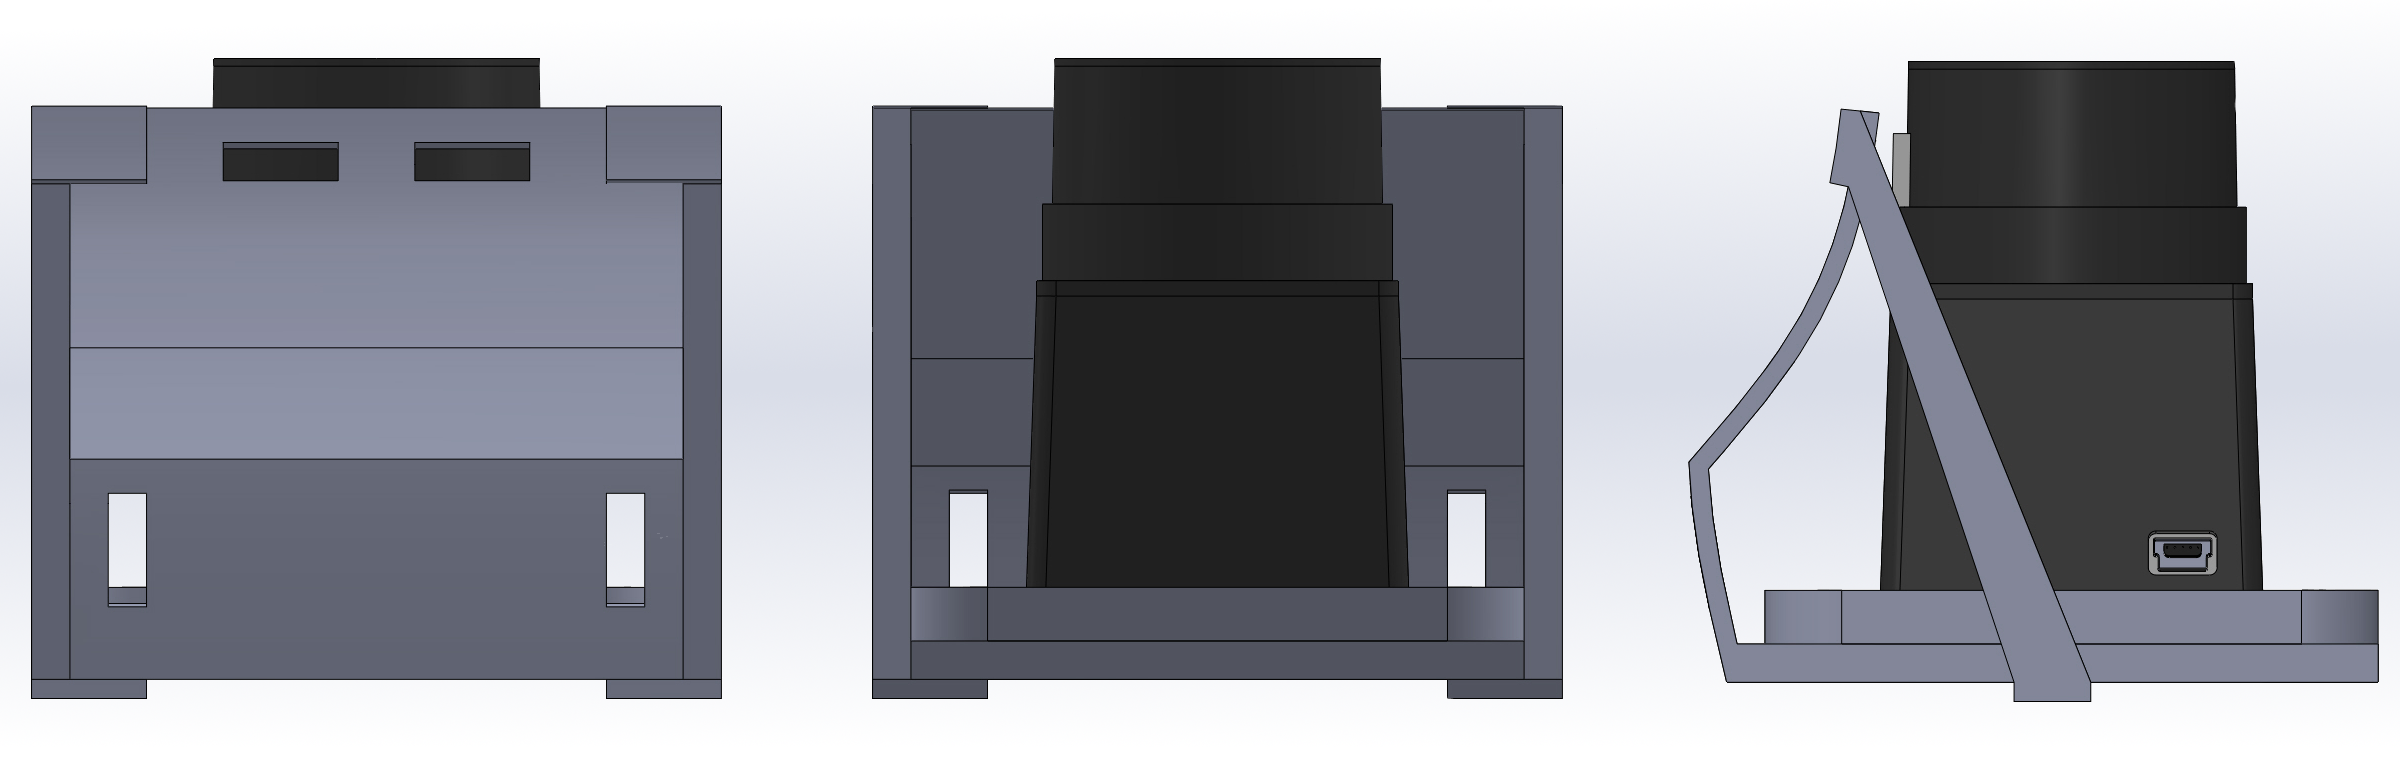
\includegraphics[width=\textwidth]{backpack/Assem_FrontOnly_Three_View1.png}
\caption{Back, front, and side views of the URG CAD model
         attached to the front subassembly of the custom mount.}
\label{fig:nao_lidar_mount_three_view1}
\end{figure}

\FloatBarrier

\paragraph{Front Plate}
The front plate has a shape that follows the form of the Nao.
It is padded with foam that is glued to the plate and absorbs vibrations.
Figure~\ref{fig:nao_lidar_mount_frontplate_trimetric1} shows a CAD model of the
front plate. It has a flat platform or tray that projects perpendicular from the 
robot to hold the base plate. 
Two mounting holes on the tray secure the base plate to the tray using bolts.
The front plate is secured to the robot via four rectangular holes which receive
velcro straps that go to the back plate. 
The top two holes are for straps that route over the shoulder of the robot while
the lower two attach waist straps.
These straps are tightened to hold the Lidar mount to the robot.

\begin{figure}
\centering
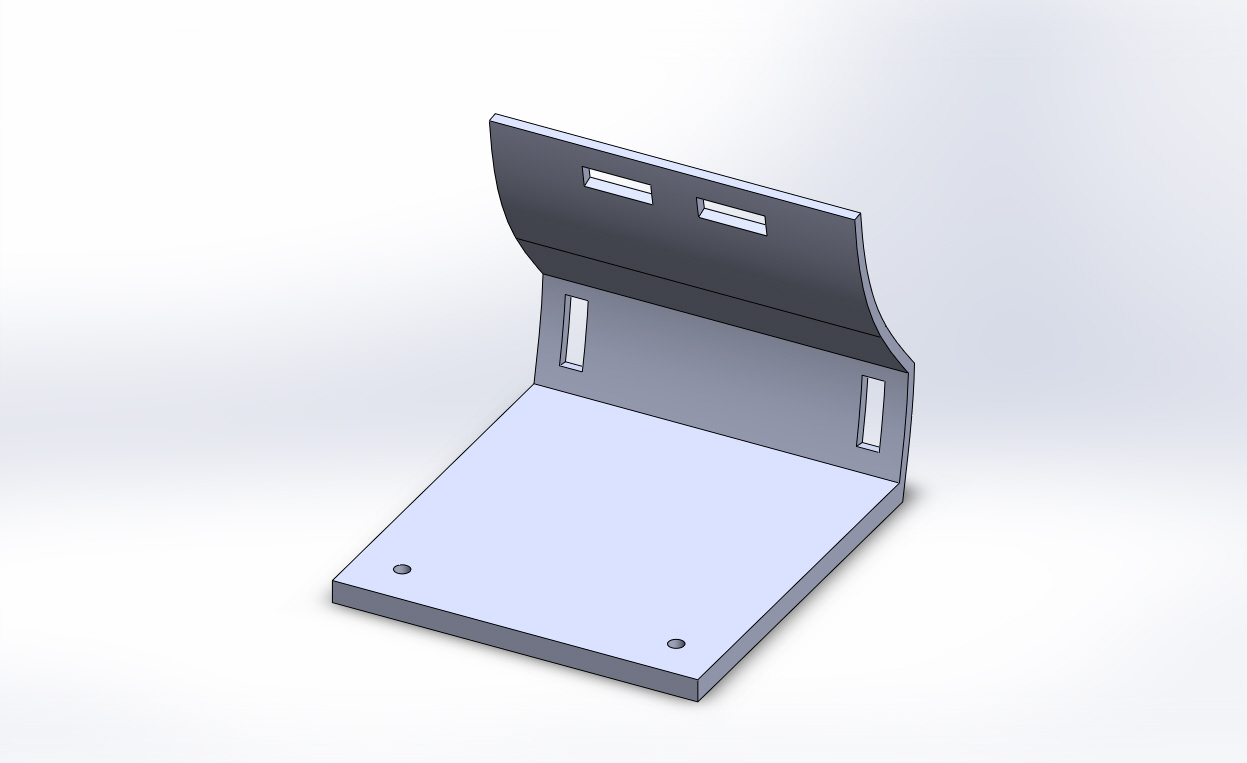
\includegraphics[height=0.25\textheight]{backpack/Front_Plate_Trimetric1.jpg}
\caption{CAD model of the front plate of the custom Lidar
         mount. The base plate and side supports attach to this plate.}
\label{fig:nao_lidar_mount_frontplate_trimetric1}
\end{figure}

\begin{figure}
\centering
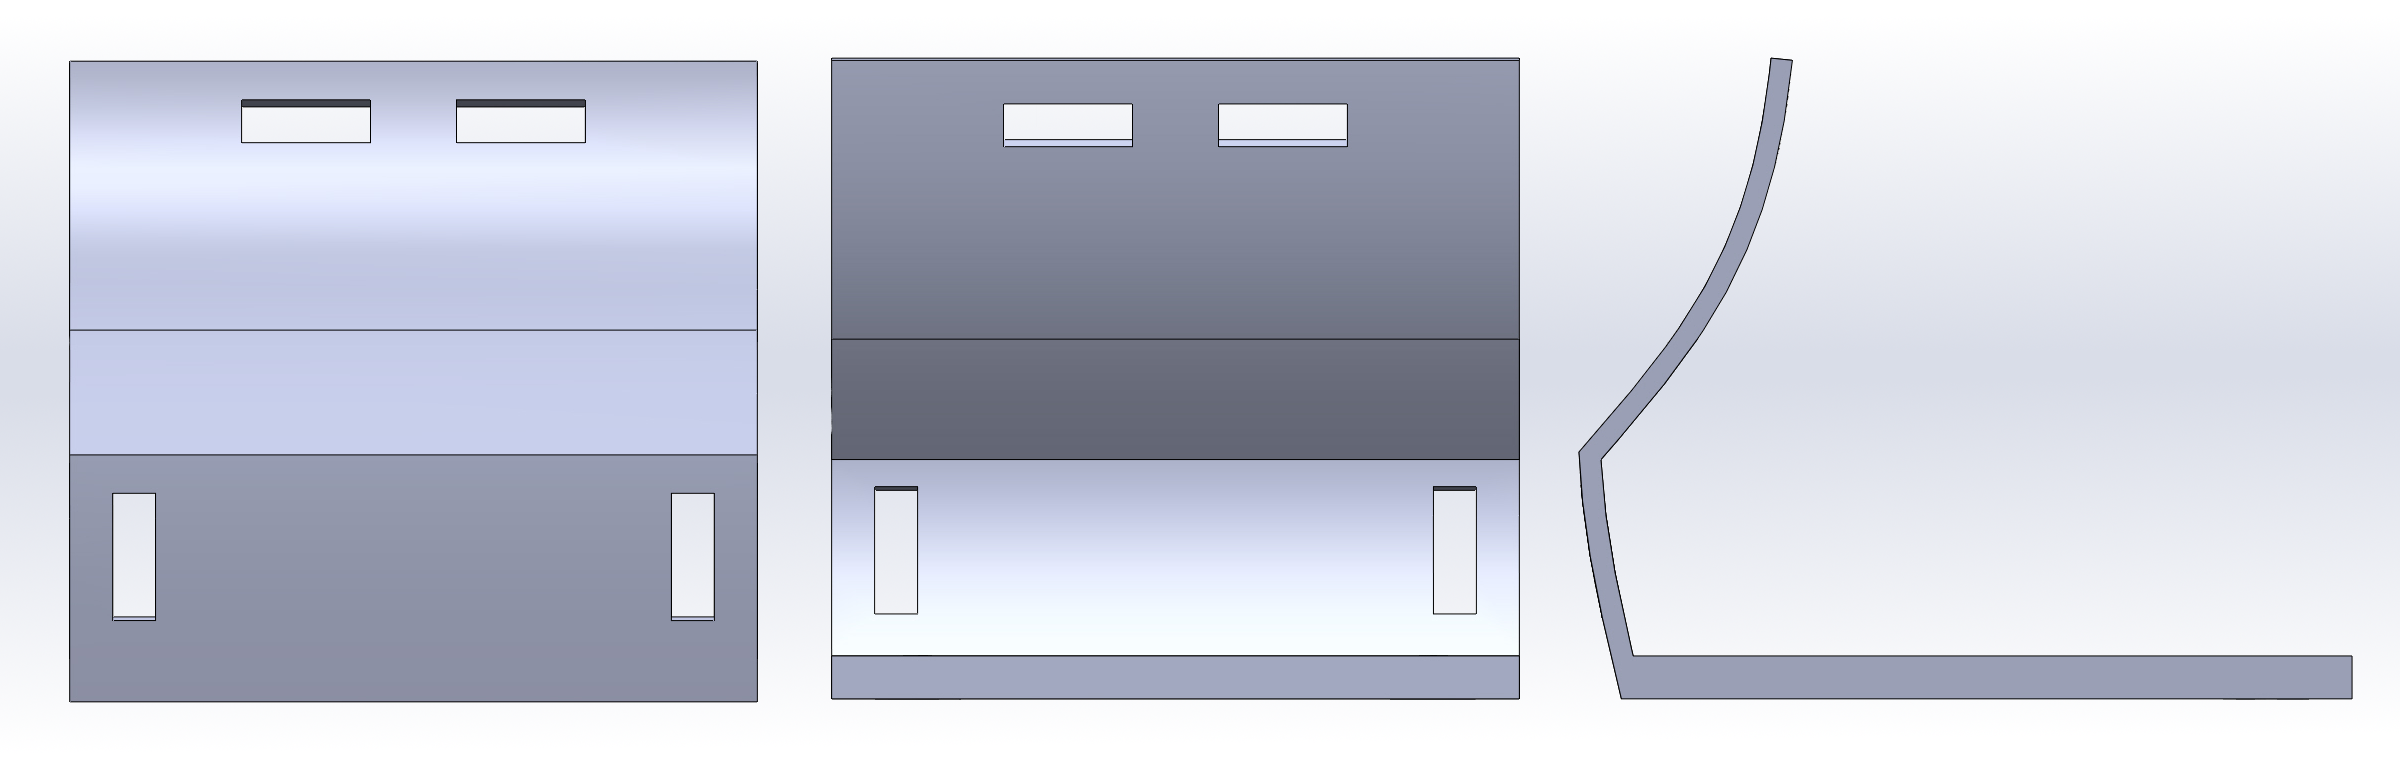
\includegraphics[width=\textwidth]{backpack/Front_Plate_Three_View1.png}
\caption{Back, front, and side views of the CAD model of the
         front plate.}
\label{fig:nao_lidar_mount_frontplate_three_view1}
\end{figure}


\paragraph{Base Plate}
The base plate is a flat piece which acts as an interface between
the URG and front plate.
The URG is attached to the base plate, which in turn is attached to the 
tray of the front plate. The URG is attached to this intermediate part
rather than directly to the front plate to facilitate the mechanical
interoperability of different sensors to the front plate without needing
to produce different front plates for different sensors. Instead, different
base plates are made for different sensors. For example, the lower cost
RPLidar \cite{rp_lidar} or the longer range VLP-16 Puck 3D Lidar
\cite{puck_lidar} are alternative Lidars that could
be mounted to the Nao for experimentation but have a different mounting 
configuration than the URG\@. In this way, new base plates can be manufactured
rather than front plates, allowing for a more modular design.

\begin{figure}
\centering
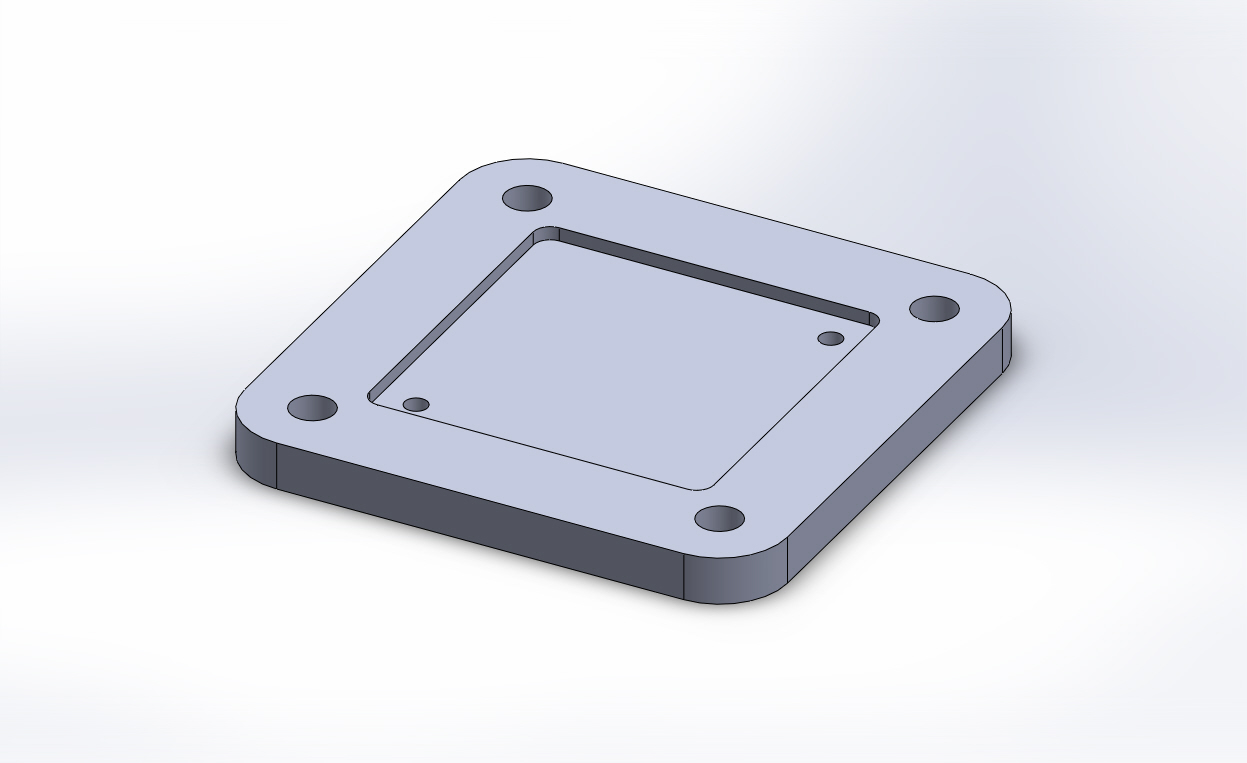
\includegraphics[height=0.25\textheight]{backpack/Base_Plate_Trimetric1.jpg}
\caption{CAD model of the base plate of the custom Lidar
         mount. The base plate is part of the front subassembly.
         The URG attaches to this plate.}
\label{fig:nao_lidar_mount_baseplate_trimetric1}
\end{figure}

Figure~\ref{fig:nao_lidar_mount_baseplate_trimetric1} shows six mounting holes
and a recessed area. Only two of the outer holes are used at a time and receive
bolts that attach it to the front plate tray. The recessed area receives the URG
and secures it to the plate using two bolts via the inner holes.

\begin{figure}
\centering
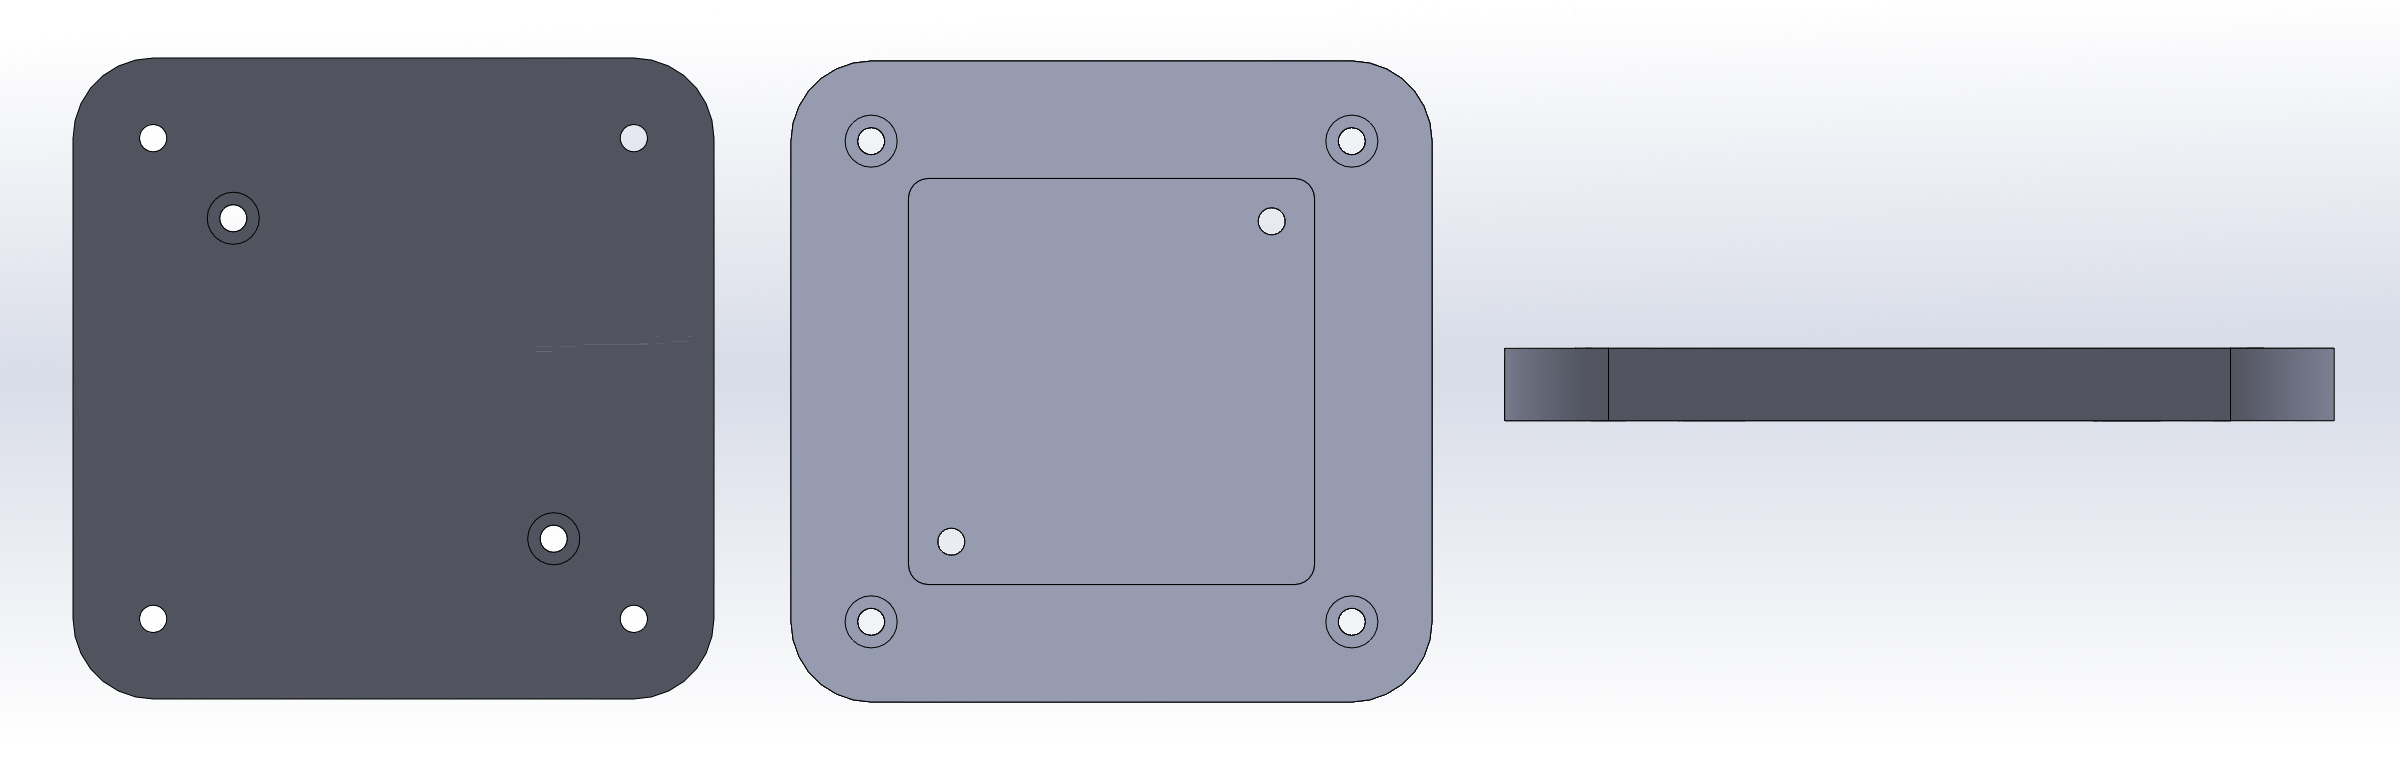
\includegraphics[width=\textwidth]{backpack/Base_Plate_Three_View1.png}
\caption{Back, front, and side views of the CAD model of the
         base plate.}
\label{fig:nao_lidar_mount_baseplate_three_view1}
\end{figure}


\paragraph{Side Supports}
The side supports act as gussets to reduce the angular deflection that can
occur with the cantilevered front plate tray. Each support has one flap
that interfaces with the underside of the tray and another that sits against
the Nao facing side of the front plate. The flaps are then bonded to the front
plate using heat. They are positioned such that as the weight of the URG pushes
down on the tray, the front-plate-to-support-flap interface will be under
compression, and the bonded joint is not as strained. This reduces the possibility
of the bonded joint being a failure mode.

\begin{figure}
\centering
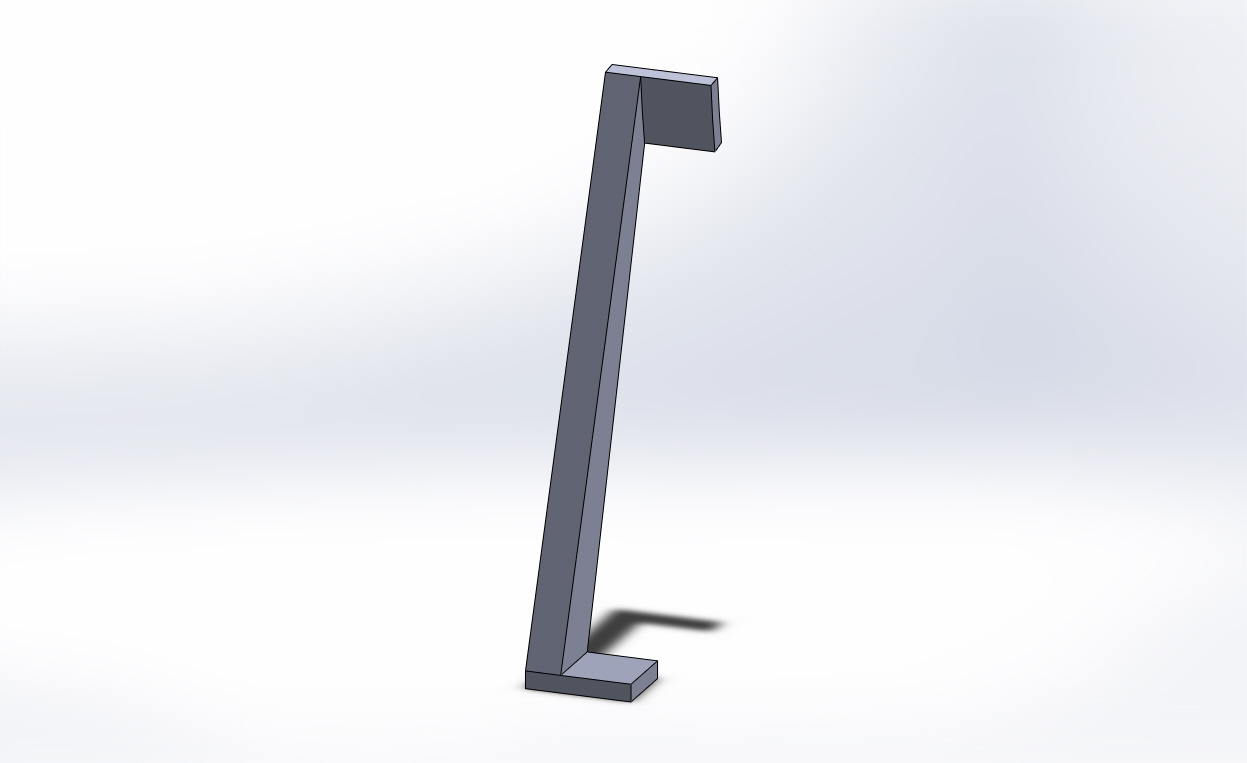
\includegraphics[height=0.25\textheight]{backpack/Support_Left_Trimetric1.jpg}
\caption{Figure showing a CAD model of the left side support of the custom
         Lidar mount. This support is bonded to the front plate to add rigidity
         to the front plate. The right side support is a mirror image of this
         part.}
\label{fig:nao_lidar_mount_supportleft_trimetric1}
\end{figure}

\begin{figure}
\centering

\includegraphics[height=0.25\textheight]{backpack/Support_Left_Three_View1.jpg}
\caption{Figure showing back, front and side views of the CAD model of the left
         side support.}
\label{fig:nao_lidar_mount_supportleft_three_view1}
\end{figure}

\FloatBarrier

\subsubsection{Back Plate}
The back plate is used to receive the straps from the front and provide another
surface to squeeze the assembly onto the robot. This ensures a large surface
area to transfer forces into the robot so no one area is stressed. It is also
lined with foam padding to better conform to the shape of the Nao.
Figure~\ref{fig:nao_lidar_mount_backplate_dimetric1} shows the plate with the
holes for the straps.
The side view seen in Figure~\ref{fig:nao_lidar_mount_backplate_three_view1}
shows how the shape conforms to the shape of the Nao. There is a large
cutout in the bottom of the plate to allow the Nao to be plugged into external
power while still wearing the assembly.

\begin{figure}[H]
\centering
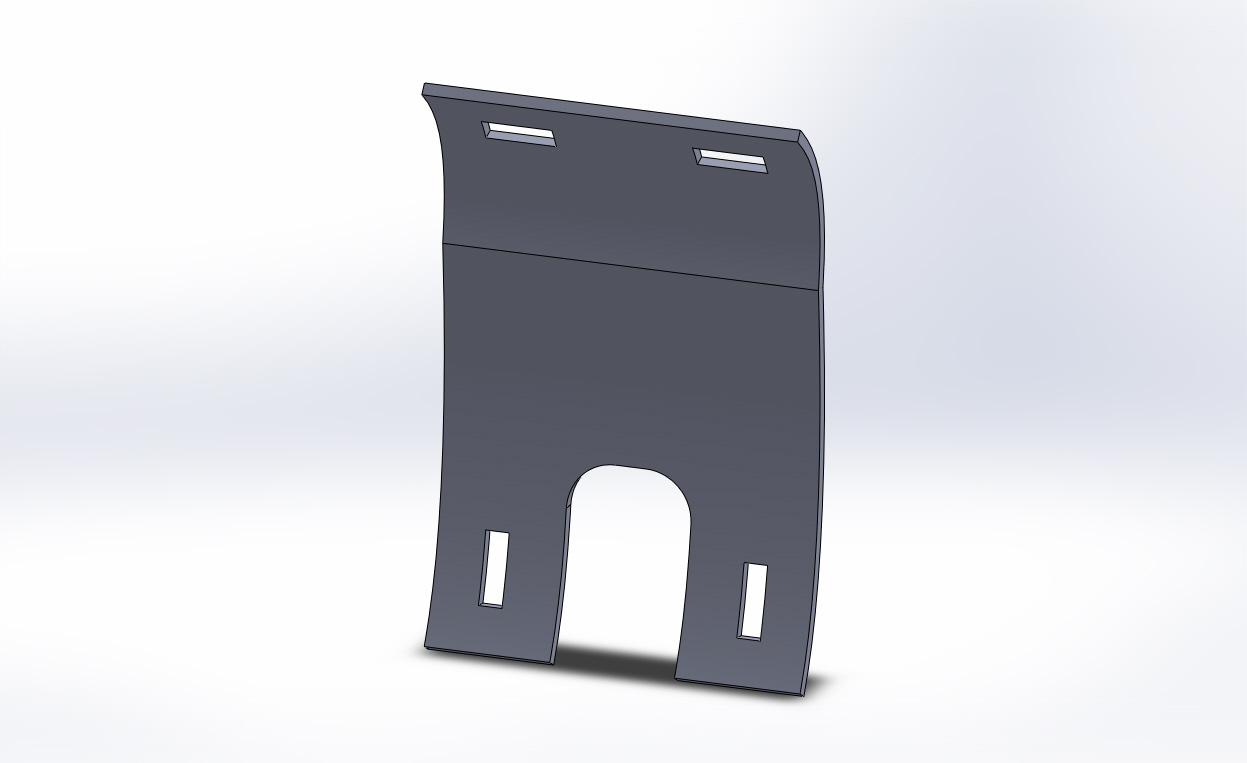
\includegraphics[height=0.25\textheight]{backpack/Back_Plate_Dimetric1.jpg}
\caption{Figure showing a CAD model of the back plate of the custom
         Lidar mount.}
\label{fig:nao_lidar_mount_backplate_dimetric1}
\end{figure}

\begin{figure}[H]
\centering
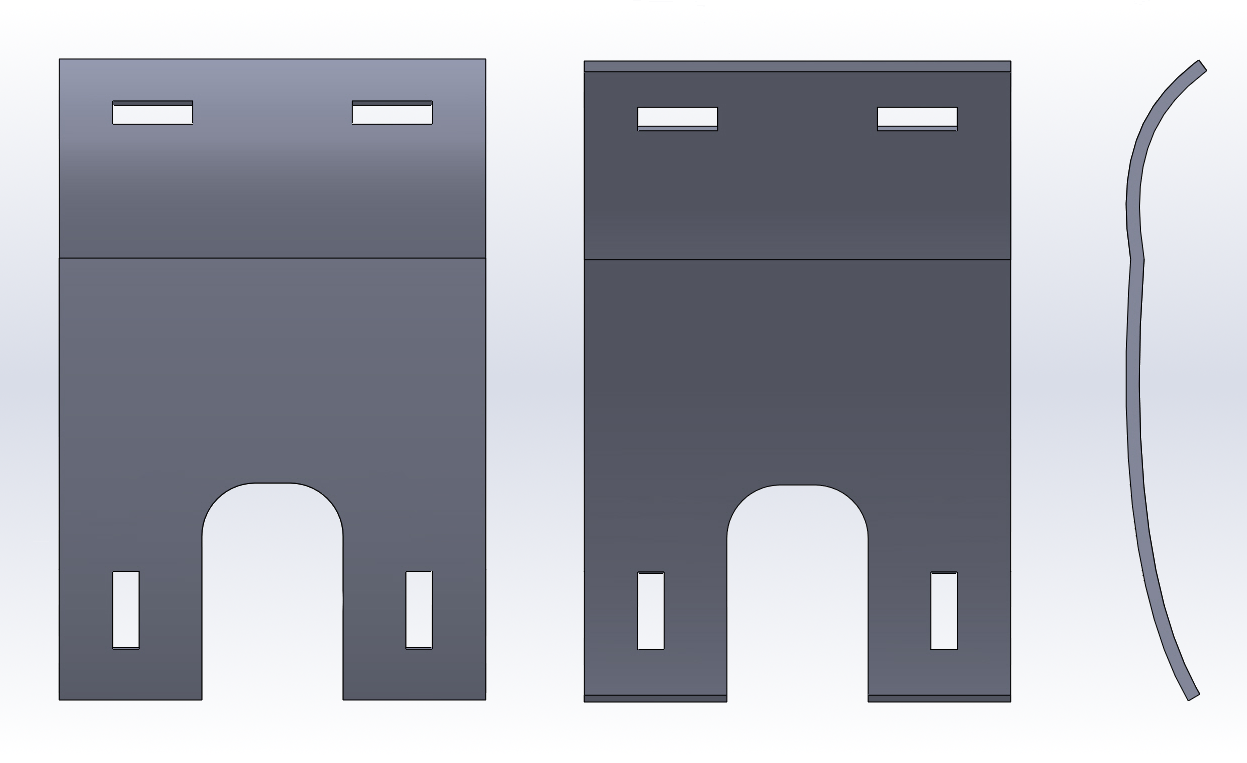
\includegraphics[width=\textwidth]{backpack/Back_Plate_Three_View1.png}
\caption{Figure showing back, front, and side views of the CAD model of the
         back plate of the custom Lidar mount.}
\label{fig:nao_lidar_mount_backplate_three_view1}
\end{figure}


